% -*- Mode: noweb; noweb-default-code-mode: R-mode; -*-
%\SweaveUTF8
\documentclass[11pt]{article}
\usepackage{graphicx}
\usepackage{Sweave}
\usepackage[utf8]{inputenc}
%% \usepackage{germanU}
%%- \usepackage[noae]{Sweave}
\usepackage[a4paper, text={14.5cm,22cm}]{geometry}
\usepackage{color} %uncomment BF
\usepackage{booktabs} % nice tables with \toprule \middlerule \bottomrule
\usepackage{amsmath} % for align
% \usepackage{wasysym} % for promille sign
% \usepackage{amssymb}
% \usepackage[textfont=it,font=small,labelfont=it]{caption}
\interfootnotelinepenalty=10000 % prevent LaTex from two-sided footnotes
\usepackage{regr-desc}

\addtolength{\textwidth}{2.5cm}%%--- 15.0 + 2.5 = 17.5
\addtolength{\oddsidemargin}{-1.04cm}

%% ================================================================

\begin{document}
\Sconcordance{concordance:regr-description.tex:/scratch/users/stahel/R/regdevelop/pkg/regr0/vignettes/regr-description.Rnw:%
1 45 1 1 7 86 1 1 5 29 0 1 3 81 1 1 2 4 0 1 3 28 0 1 2 103 1 1 2 3 0 1 %
4 12 0 1 2 16 1 1 2 15 0 1 3 4 0 1 2 100 1 1 4 5 0 1 3 204 1 1 6 5 0 1 %
3 94 1 1 6 5 0 1 3 76 1 1 2 5 0 1 3 21 1 1 2 1 3 13 1 2 3 99 1}

\setkeys{Gin}{width=1\textwidth}
\baselineskip 15pt

\title{\vspace*{-10mm}
The R-Function \T{regr} and Package \T{regr0} for an Augmented 
Regression Analysis}
\author{Werner A. Stahel, ETH Zurich}
\maketitle

\begin{abstract}\noindent
The R function \T{regr} is a wrapper function that allows for fitting
several different types of regression models by a unified call, and
provides more informative numerical and graphical output than the 
traditional \T{summary} and \T{plot} methods.
The package \T{regr0} contains the functions that go along with 
\T{regr} and a number of others.
It is written to make data analysis more effective by providing
user-oriented, flexible functions.
It is available from \T{R-forge} and is still in development.
\end{abstract}

\section{Introduction}

Regression models are fitted in the statistical programming environment R 
by diverse functions, depending on the particular type of model.
Outputs obtained by calling the function \T{summary} on the object produced
by the fitting function look often quite similar. Graphical output for
residual analysis is obtained by calling \T{plot}, but the result is not
always informative. 

The function \T{regr} allows for fitting various regression models
with the same statement, provides a more informative numerical output
and enhanced plots for residual analysis. 

\T{regr} proceeds by 
checking arguments, then calling the suitable fitting method from standard
R or other packages,
collecting useful statistics from the resulting object and a call of 
\T{summary} on it and adding a few to generate an object of class
\T{regr}. 
%%- The printing method for these objects shows the results that are usually 
%%- of interest.
%%- The plotting method produces a much more complete set of residual plots
%%- than the plotting methods for the usual fitting objects do.


In particular, the following models can be fitted by \T{regr}:
\begin{itemize}
\item 
  ordinary linear models, using Least Squares or robust estimation,
  by calling \T{lm} or \T{lmrob} from the \T{robustbase} package,
\item
  generalized linear models, by calling \T{glm},
\item
  multinomial response models, by calling \T{multinom} of package
  \T{nnet},
\item
  ordered response models, by calling \T{polr} of package
  \T{MASS},
\item
  models for survival data and Tobit regression, by calling
  \T{survreg} or \T{coxph} of package \T{survival},
\item
  multivariate ordinary linear models, by calling \T{lm}
\item
  nonlinear models, by calling \T{nls}
\end{itemize}

This document presents the main features of the package \T{regr0}
and explains the ideas behind them. 
It gives no details about the functions. They can be found in
the help files.

The package is available from \T{R-forge}, e.g. by calling\\
\T{install.packages("regr0", repos="http://r-forge.r-project.org")}.\\
The reason why it is not on CRAN and why it is called \T{regr0} rather than 
\T{regr} is that the author is still developing additional features and
does not yet want to guarantee upward compatibility.
It also means that comments and suggestions are very welcome:
\T{stahel\@ stat.math.ethz.ch} %% !!! at

\section{Numerical Output}
The useful numerical output of fitting functions is usually obtained by
calling \T{summary} on the object produced by the fitting method.
This results, for most functions, in a table showing the estimated
regression coefficients, their standard errors, the value of a test
statistic (t or z or deviance) and, for the 
ordinary linear model, a p value for the tests for zero coefficients. 
It is followed by an overall summary, usually including a test for
the hypothesis that all coefficients are zero, and a standard deviation of
the error and coefficient of determination, if applicable.

If there are factors (qualitative explanatory variables) in the model, 
the coefficients are not always interpreted adequately, and the 
respective standard errors, t and p values are of little use and often
misinterpreted. 
On the other hand, the information whether a factor has a significant
effect is not available from the summary but has to be obtained by calling 
\T{drop1} on the fit object. 
(The function \T{anova}, which seems to be suited according to its
name, usually does not answer this question.)

This situation cannot be called user friendly.
The function \T{regr} is meant to provide the results that are needed
without having the user call different functions and select the 
output that is safe to be interpreted.

Here is a result of printing a \T{regr} object.
\begin{Schunk}
\begin{Soutput}
  Blasting for Tunnel Excavation 

Call:
regr(formula = logst(tremor) ~ location + log10(distance) + log10(charge), 
    data = d.blast)
Fitting function:  lm 

Terms:
                  coef stcoef df signif p.symb
(Intercept)      2.971     NA  1  13.37     NA
location            NA     NA  7   3.48    ***
log10(distance) -1.506 -0.790  1 -12.13    ***
log10(charge)    0.623  0.406  1   8.17    ***
---
Signif. codes:  0  ***  0.001  **  0.01  *  0.05  .  0.1     1  

St.dev.error:  0.141   on 352 degrees of freedom
Multiple R^2:  0.798    Adjusted R-squared: 0.793 
F-statistic:    155   on 9 and 352 d.f.,  p.value: 1.55e-116 

Coefficients for factors:
$location
  loc1        loc2        loc3        loc4        loc5        loc6       
  -0.0174      0.1334 ***  0.1125 *** -0.1829 *** -0.0511 *    0.0530 *  
  loc7        loc8       
  -0.0315     -0.0160    
\end{Soutput}
\end{Schunk}

\subsection{Standard output for continuous explanatory variables}
The ``Terms:'' table characterizes the effects of the individual terms in
the model. For continuous explanatory variables (the last 2 lines in the
example) it shows:
\begin{description}
\item[\T{coef},] the estimated value of the coefficient;
\item[\T{df},] degrees of freedom, $=1$ for continuous variables;
\item[\T{ciLow, ciHigh},] the limits of the confidence interval;
\item[\T{R2.x},] the coefficient of determination for regressing 
  the explanatory variable in question on the other terms in the model.
  This is one of the wellknown collinearity diagnostics.
\item[\T{signif},] a significance measure that is $>1$ for estimated
  coefficients differing significantly from 0, see below for its
  definition;
\item[\T{p.value},] the p value for testing if the coefficient could be
  zero. 
\item[\T{p.symb},] the usual significance symbols.
\end{description}
In fact, 2 more columns are contained in \T{rr\$termtable}, but they are
not printed by default:
\begin{description}
\item[\T{se},] the standard errors of the estimated coefficients; 
\item[\T{stcoef},] the estimated standardized coefficient,
  defined as \T{coef} times the standard deviation of the explanatory
  variable, divided by the standard deviation of the response (if
  the response is continuous as assumed here), see below for its use;
\end{description}
\Tit{User options.}
The default for the columns to be printed is set by an option stored 
in the \T{UserOptions} list and controled by the function 
\T{userOption} in the same way that the usual options are
controled by the function \T{options}.

\Tit{Significance}
The usual \T{summary} output of fitting functions includes the 
t (or z) values of the coefficients as a column in the coefficients 
table. 
They are simply the ratios of the two preceding columns. 
Nevertheless, they provide a kind of strength of the significance of the
coefficients. The p value may also serve as such a measure, but it is less 
intuitive as it turns tiny for important variables, making comparisons
somewhat more difficult than t values. 
The significance of t values depends on the degrees of freedom, but
informed users will know that critical values are around $\pm2$, and they will
therefore informally compare t values to $\pm2$. 
Based on these considerations, we introduce a new measure of significance
here. 

The new significance measure is defined as
\[
  \T{signif} = \T{t value}\;/\; \T{critical value}
\]
where \T{critical value} is the critical value $q_{df}$ of the 
t distribution and depends on the degrees of freedom of the residuals. 
%%- The definition is applicable for continuous explanatory
%%- variables as well as for binary factors.
%%- For other factors, we will extend this definition below.

\Tit{Confidence Intervals.}
The standard errors provided by the usual \T{summary} tables allow for
calculating confidence intervals for continuous explanatory variables,
by the formula $\T{coef} \;\pm\; q_{df}\cdot\T{std.error}$.
By default, they are shown in the Terms table. 
If the table gets too wide, the confidence limits may be suppressed.
They can then be calculated as
%%- The formula based on \T{signif} is
\[
  \T{coef}\cdot\;(1\pm\;1/\T{signif}\;)
\]
This is slightly more complicated for a calculation in the mind than
\T{coef}$\pm 2$\T{se}, 
but the formula shows an additional interpretation of \T{signif} 
in terms of the confidence interval:
If the input variable were scaled such that the confidence interval had 
half width 1, then the estimate would be \T{signif} units away from zero.

\Tit{Standardized Coefficients}
Standardized coefficients are meant to allow for a comparison of the 
importance of explanatory variables that have different variances.
They are also stored in \T{rr\$termtable} as the column \T{stcoef}.

\begin{Schunk}
\begin{Soutput}
 [1] "coef"    "se"      "ciLow"   "ciHigh"  "df"      "testst"  "signif" 
 [8] "p.value" "p.symb"  "stcoef"  "R2.x"   
\end{Soutput}
\begin{Soutput}
  Blasting for Tunnel Excavation 

Call:
regr(formula = logst(tremor) ~ location + log10(distance) + log10(charge), 
    data = d.blast)
Fitting function:  lm 

Terms:
                  coef stcoef df signif p.symb
(Intercept)      2.971     NA  1  13.37     NA
location            NA     NA  7   3.48    ***
log10(distance) -1.506 -0.790  1 -12.13    ***
log10(charge)    0.623  0.406  1   8.17    ***
---
Signif. codes:  0  ***  0.001  **  0.01  *  0.05  .  0.1     1  

St.dev.error:  0.141   on 352 degrees of freedom
Multiple R^2:  0.798    Adjusted R-squared: 0.793 
F-statistic:    155   on 9 and 352 d.f.,  p.value: 1.55e-116 

Coefficients for factors:
$location
  loc1        loc2        loc3        loc4        loc5        loc6       
  -0.0174      0.1334 ***  0.1125 *** -0.1829 *** -0.0511 *    0.0530 *  
  loc7        loc8       
  -0.0315     -0.0160    
\end{Soutput}
\end{Schunk}
Each of them shows the effect on the response of increasing ``its'' 
carrier $X^{(j)}$ by one standard deviation, as a multiple 
of the response's standard deviation. 
This is often a more meaningful comparison of the relevance of the input
variables. 

Note, however, that increasing one $X^{(j)}$ without also changing
others may not be possible in a given application, and therefore, 
an interpretation of coefficients can always be tricky.
Furthermore, for binary input variables, increasing the variable by one
standard deviation is impossible, since an increase can only occur from 0
to 1, and therefore, the standardized coeffient is somewhat 
counter-intuitive in this case.

\subsection{Factors}
For factors with more than two levels, (\T{location} in the example), there
are several coefficients to be estimated. 
Their values depend on the scheme for generating the 
dummy variables characterizing the factor, which is determined 
by the \T{contrasts} option (or argument) in use.
We come back to this point below (``Contrasts'').

Note that for factors with only two levels, the problem does not arise,
since the single 
coefficient can be interpreted in the straightforward manner as 
for continuous explanatory variables. \T{regr} therefore treats binary
factors in the same way as continuous explanatory variables.

The test performed for factors with more than two levels, which is shown 
in the \T{Terms} table by the \T{p.value} entry, 
is the F test for the whole factor (hypothesis: all coefficients are 0). 
It is obtained by calling \T{drop1}.
The significance measure is defined as 
\[
  \T{signif} = \sqrt{\T{F value}\;/\;q_{df1,df2}}
\]
where $q_{df1,df2}$ is the critical value of the F distribution.
It reduces to the former one for binary factors.

The collinearity measure \T{R2.x} for factors is a formal generalization of 
\T{R2.x} for terms with one degree of freedom, determined by applying
the relationship with the ``variance inflation factor'',
\T{R2.x}$=1/(1-\mbox{vif})$ to the generalized vif. 
[More explanation planned.]

\Tit{All coefficients for factors.}
The usual contrast option \T{contrasts=\penalty-100%
"contr.treatment"} gives the coefficients of the dummy variables 
a clear interpretation: 
they estimate the difference of the response between level $k$ and 
level 1 for $k>1$.
Another popular setting is \T{contrasts=\penalty-100%
"contr.sum"}, for which the $k$th coefficient estimates the effect 
of the $k$th level in such a way that the sum of all coefficients is 0.
For this setting, the last of these effects is not given in the
vector of coefficients, \T{rr\$coef}.

In order to avoid ambiguities, the \T{regr} output lists the 
estimated effects for all levels of the factors after the term table.
Even though the interpretation of significance and confidence intervals of
the individual effects of the levels is delicate, \T{regr} objects include
a full table, similar to the term table explained above, for each factor.
By default, however, only the estimated effects ar shown, together with the
``star symbols'' for their significance.

\Tit{Contrasts.}
An advantage of \T{contr.sum} over the usual \T{contr.treatment}
contrasts is that it avoids the (often unconscientious) choice of a
reference level -- the first level -- and allows, for each level, 
to assess immediately how large its effect is as compared to an overall
average effect.
An even more important advantage appears when interactions between factors
are included in the model: 
The main effects of one factor, including its significance, 
may still be interpreted (with caution) as average effects over the
levels of the other factor.

The \T{contr.sum} setting is not well adapted to unbalanced factors, since
the unweighted sum of coefficients is forced to be 0.
This leads to large standard errors when one of the levels has a low 
frequency. 
The \T{regr0} package provides the option \T{contr.wsum} for which the
sum of coefficients weighted with the frequencies of the levels is zero.
This type of contrasts is the default in \T{regr0}.

\subsection{Model summary}
The last paragraph of the output gives the summary statistics.
For ordinary linear models, the estimated standard deviation or the error
term is given first. (It is labelled ``Standard error of residual'' in the 
\T{lm} output, which we would label a misnomer.)
The \T{Multiple R\^{}2} is given next, together with its ``adjusted''
version, followed by the overall F test for the model.

For generalized linear models, the deviance test for the model is given.
If applicable, a test for overdispersion based on residual deviance is also
added. 

\subsection{Model Comparisons}
When model development is part of the statistical analysis, it is useful to
compare the terms that occur in different models under consideration.
There is a function called \T{modelTable} that collects coefficients, 
p values, and other useful information, and a \T{format} and \T{print} 
method for showing the information in a useful way.

\begin{Schunk}
\begin{Soutput}
[1] "no"       "datetime" "device"   "charge"   "distance" "tremor"   "location"
\end{Soutput}
\begin{Soutput}
                               r.blast       r.blast2    
(Intercept)                     2.9706        2.8048     
location                          +++   ***     +++   ***
log10(distance)                -1.5062  ***  -1.3548  ***
log10(charge)                   0.6226  ***   0.7507  .  
location:log10(distance)           -            +++   ***
location:log10(charge)             -            +++   .  
log10(distance):log10(charge)      -         -0.1085  .  
.sigma.                         0.1409        0.1358     
.df.                              10            25       
\end{Soutput}
\end{Schunk}

\subsection{Model Selection}
The well-known functions \T{drop1} and \T{add1} are adapted by 
providing additional methods. 
The function \T{drop1} has a useful default for the argument (\T{scope}):
It incluses all terms that can be sendsibly dropped from the model.
This is not provided for the base version of \T{add1}. 
This latter function is very useful to check whether squared continuous
variables or interactions between variables should be included into the
model. Therefore, our version of \T{add1} provides this default \T{scope}
(calculated by \T{terms2order}),
and both \T{drop1} and \T{add1} calculate F tests in addition to AIC.

Since \T{drop1} and \T{add1} methods are available, \T{step} can be used to
select a model automatically. The default \T{regr} version chooses ``both''
directions, bakward and forward, and extends the \T{scope} as in \T{add1}.

\begin{Schunk}
\begin{Soutput}
Single term additions

Model:
logst(tremor) ~ location + log10(distance) + log10(charge)
                              Df Sum of Sq  RSS   AIC F value  Pr(>F)    
<none>                                     6.99 -1409                    
I(log10(distance)^2)           1     0.003 6.98 -1407    0.15   0.700    
I(log10(charge)^2)             1     0.143 6.84 -1415    7.35   0.007 ** 
location:log10(distance)       7     0.726 6.26 -1435    5.72 2.8e-06 ***
location:log10(charge)         7     0.112 6.87 -1401    0.80   0.585    
log10(distance):log10(charge)  1     0.000 6.99 -1407    0.01   0.929    
---
Signif. codes:  0 ‘***’ 0.001 ‘**’ 0.01 ‘*’ 0.05 ‘.’ 0.1 ‘ ’ 1
\end{Soutput}
\begin{Soutput}
logst(tremor) ~ location + log10(distance) + log10(charge)
<environment: 0x55b4013bba00>
\end{Soutput}
\end{Schunk}

The usual stopping rule for stepwise model selection relies on the AIC
criterion. Note that there is a funny argument for this choice:
The former stopping rule, which aimed at keeping only formally
``significant'' terms in the model has been criticized because of the
multiplicity problem: The retained terms appear more significant than they
are, because they are the most significant of an unspecified number of
candidates. Thus, the formal significance tests for the terms are liberal
to an unknown degree, and the selected models tend to be too large.

Therefore, a new criterion was introduced, the AIC (or the BIC).
Its justification is based on optimization of a prediction error sum of 
squares. It should be noted that it leads to larger models than the
significance criterion. Thus, one should expect to see non-significant
terms in the selected model, even based on the liberal formal tests
provided in regression outputs.

Unfortunately, it is not possible to specify the stopping criterion 
in \T{step}. However, it can be shown that setting its argument \T{k=5},
one usually obtains the model with the formally significant terms.


%\pagebreak
\Vneed{50mm}
\section{Residual Analysis}
%\subsection{Basic plot methods.}
The residual plots that are produced by plotting an \T{lm} or \T{glm}
object are: 
\begin{itemize}
\item 
The Tukey-Anscombe plot showing residuals against fitted values,
which is certainly the most important single diagnostic tool for assessing
model assumptions;
\item
The Scale plot, which shows square-root transformed absolute values of
residuals against 
fitted values and helps to spot unequal variances (if these depend on the
expected value of the response).
\item
The normal quantile-quantile plot, which makes sense only for ordinary
linear models and in some cases for generalized linear models. 
It is not essential since skewness and outliers can also be seen in the
Tukey-Anscombe plot if they are relevant;
\item
The leverage plot, displaying residuals against leverage values.
This plot is useful to detect influential observations.
\end{itemize}

\subsection{What \T{plot.regr} does}
The plotting method for \T{regr} objects has many addtional features, to be
described in more detail in the following subsections.
\begin{itemize}
\item
The set of plots that is shown by default is adjusted to the type of
model. A normal QQ-plot of residuals is only shown if appropriate.
If weights are used, the residuals divided by the weight 
are also plotted against the
weights, which helps to see if the weighting rule was adequate.
\item 
Most importantly, residuals are plotted against explanatory variables.
This can also be achieved by calling \T{termplot} for other fit objects,  
but experience shows that this is often neglected by average users.

Residuals can be plotted easily against the index (sequence
number) of the observation, since this may show trends or 
correlations of errors in time, if the sequence reflects time.
\item
The plots are augmented by a smooth line fitted to them -- which is also
available in the classical R functions -- and two additional smooth lines
that allow to judge the scale dependence on the variable shown.
In addition, simulated smooths are added in order to assess an informal 
``significance'' of curvature in the smooth of the data. 
Furthermore, a reference line is given, which helps finding
an appropriate modification of the model if significant curvature is
found. 
\item
Finally, plotting methods are defined for models for which no useful 
methods are available in the basic R packages, notably ordered response
regression and censored responses.
\end{itemize}

The number of plots produced by calling \T{plot} on a \T{regr} object may
be elevated. The arguments \T{plotselect} and \T{xplot} allow for 
requiring or deselecting any of them. 
The arguments to \T{plot.regr} are numerous and allow for varying many
features, including those for which the default behavior is discussed below.

The plotting pages are marked in the right lower corner by the date and a
project title and step label, if available from \T{options}. 
(This \T{stamp} can be suppressed by setting \T{userOptions(stamp=FALSE)}.) 

The default plotting character is a plus sign. Its size is adjusted to
the number of points.

The usual set of plots can be seen by executing the examples on
\T{help('plot.regr')}. 
A single plot is shown here for easy reference in the following
descriptions. 

\begin{figure}[htb]
%% \centerline{\includegraphics[width=1\textwidth]{p-plotregr-ta}}
\begin{Schunk}
\begin{Soutput}
[1] "plot.regr done"
\end{Soutput}
\end{Schunk}
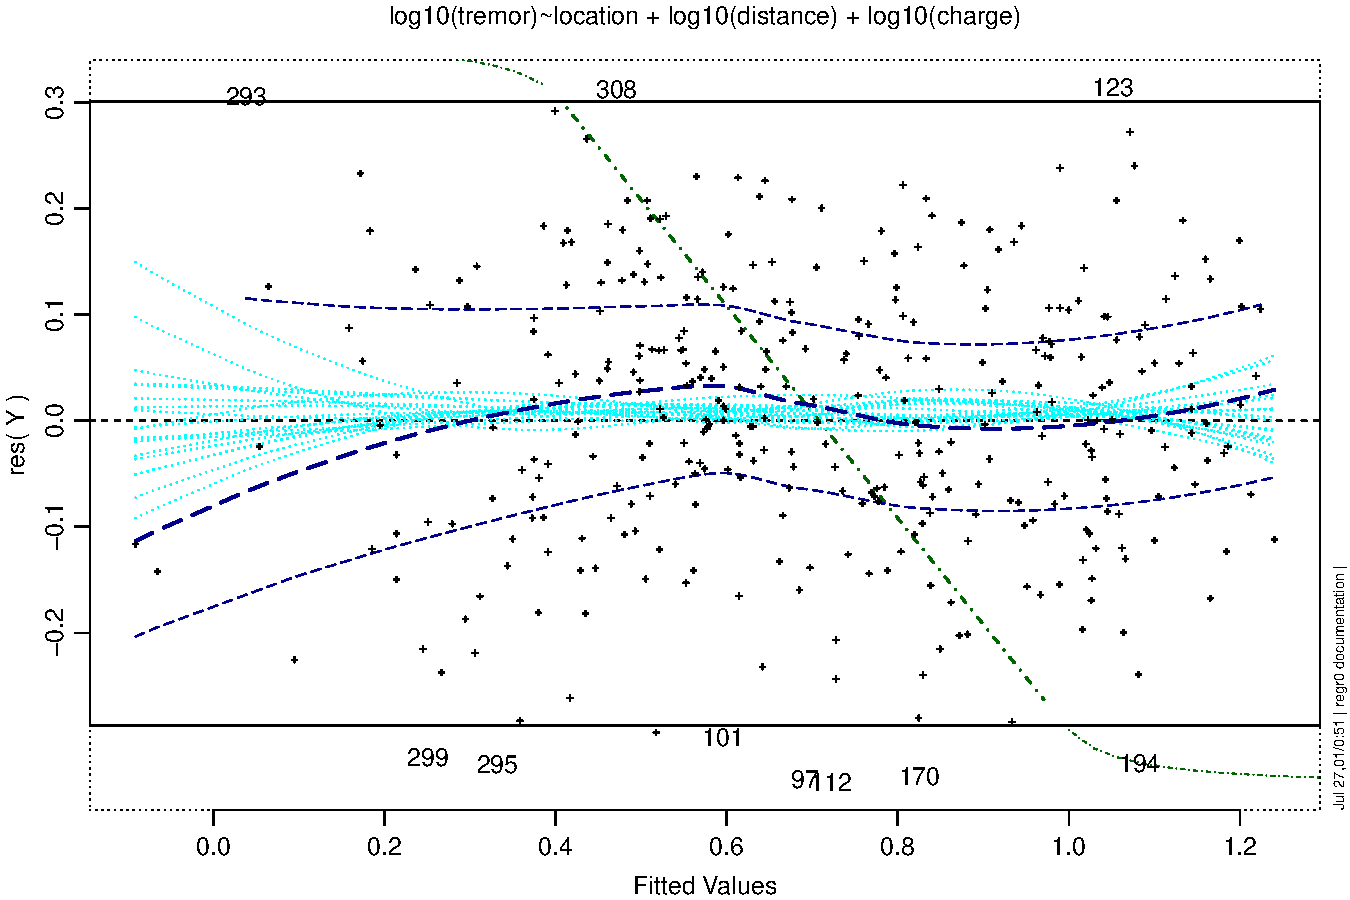
\includegraphics{regr-description-taplot}
\caption{A Tukey-Anscombe plot.}
\end{figure}

\subsection{Extreme Residuals}
If there are one or a few outliers in any plot, the structure of the
majority of the data becomes more difficult to grasp. 
Therefore, the \T{plot} method first flags outliers in the residuals.
If there are any, the range of the vertical axis is split into an
``ordinary plotting range'', where the non-outliers appear as usual, and
an ``outlier margin'', where the outliers are shown on a highly nonlinear
scale that maps the range from the limit of the ordinary range to infinity 
to this margin.

In order to ease identification, a suitable number of most extreme
residuals are labeled with their \T{row.names} (by default).

%%!!! bis hierher durchgelesen 1609

\subsection{Smooths}
Fitting a smooth (blue dashed line in the Figure) 
to a residual scatterplot helps to spot a potential
nonlinearity of the relationship between the response and the variable
shown in the plot -- the fitted values or a single explanatory variable.
The smooth used by default is \T{loess} with a span depending on the number
of observations (currently $= 5n^{-0.3}$ for ordinary regression, and twice 
this number for generalized linear regression; do not ask why).
Such a smooth is more essential for generalized linear models than for 
ordinary ones, since artefacts of the residuals may make it impossible to 
see curved relationships from a display of the residuals.

It is difficult to decide if a smooth line is curved ``significantly'',
such that searching for a better model should be helpful instead of most
probably leading to overfitting the data.
In order to help judging the ``natural curvature'', 19 sets of data are
generated by 
%drawing random response values according to the fitted model.
re-randomizing the residuals. 
The smooths obtained for these sets are also shown (in light blue in the
Figure -- I hope that this can be seen in all versions of this document).
If the smooth determined from the data is clearly the most extreme in some
aspect, one may conclude that the model does not fit adequately.
The number 19 is chosen to correspond to a ``significance level'' of 5\%.
Up to now, such simulated datasets are only generated for ordinary linear
and for generalized linear regression. 

In addition to the smooth line that fits the center of the residuals,
there is a line characterizing the two other quartiles. 
It is obtained by first calculating the deviations from the smooth line,
then fitting a smooth line each through the positive and through the
negative deviations, and finally adding the central smooth back to these
two fits.
These lines facilitate to check the overall symmetry and the
homoscekasticity of the residuals.

\subsection{Augmented Tukey-Anscombe Plot}
The plot of residuals against fitted values is the most important
diagnostic tool to assesss the validity of model assumptions.
It allows for detecting deviations from linearity, homoscedasticity,
symmetry and normal distribution of the random deviations.

If there is curvature, one remedy may be to transform the response
variable. This can help only if the relation between fitted and
response values is monotone -- otherwise, quadratic terms are the
most straightforward modification of the model.
Monotonicity is easy to see if the response is plotted on the vertical
axis instead of the residuals.
This display can also be requested from \T{plot.regr}
(by setting \T{plotselect=c(yfit=3)}).

In order to avoid the necessity to either call \T{plot} again or to 
ask for the plot of response against fitted values routinely,
a \ul{reference line} (green dot-dashed line in the Figure)
is shown in the Tukey-Anscombe plot.
It connects points with equal response values. Since the response can be
determined by adding the two coordinates of the plot -- 
fitted plus residual -- lines of equal response values have slope -1.
The reference line shown is such a line, the one going through the center
of the points in the plot.
If the smooth never gets steeper than the reference line, then the
suggested relation between fitted and response values is monotone, and a
transformation of the response may remove the non-linearity.

One might argue that a plot of the response on the fit is more
straightforwardly interpreted than the Tukey-Anscombe plot with the
reference line. We think that the Tukey-Anscombe plot can show the
deviations from model assumptions more clearly and should therefore be
preferred, and that the reference line, after a short learning period, will
be easy enough to work with and helps avoiding an additional display. 
Of course, some users may disagree.

\subsection{Scale Plot}
The absolute values of the \emph{standardized} residuals are plotted
against the fitted values 
in order to see more clearly than in the Tukey-Anscombe plot whether the 
scatter of residuals depends on the expected values.
The plot shown when plotting \T{lm} objects uses square roots of absolute
residuals instead of the absolute values themselves because they are more
symmetrically distributed. This appears as a technical argument to me and
it may confuse unexperienced users. While square roots are therefore
avoided for plotting, they are still used to calculate the smooth that is
added to the plot.

When the smooth line in the Tukey-Anscombe plot indicates a curved
relationship, the residuals contain a bias, and deviations from a straight
line in the scale plot are not necessarily an indication of
heteroscedasticity. On the other hand, clear differences in the scatter
around the smooth line in the Tukey-Anscombe plot may not show up in 
the scale plot as a consequence of the bias.
Therefore, \T{plot.regr} uses modified residuals to generate the scale
plot: The difference between the residual and the smooth fit in the
TA plot is this modified residual, of which the absolute value is used.

\subsection{QQ-Plot}
The QQ-normal plot of residuals only makes sense in the ordinary linear or
nonlinear regression. It is therefore avoided by default for other models 
(unlike in standard R).
Furthermore, this plot only makes sense if quantities with the same normal
distribution are used to generate it. 
Therefore, standardized residuals should be used.
The preceding reasoning for using modified residuals also applies.
In fact, these modified residuals are modified again to reflect the
potentially different scales: they are divided by the value of the smooth
in the scale plot before they are used for the QQ-plot.

\subsection{Weights}
If weights are given by the user, they should usually reflect different
variances of the random errors $E_i$, and the residuals, multiplied by the
square root of the weights, should have constant variance.
The standardized absolute residuals are therefore plotted against the weights.
If the size of these residuals is not constant but depends on the weight, 
the rule or weighting function should be revised.

If weights are given, they are also used as the sizes of the plotting
symbols (circles) in other plots.

\subsection{Leverage Plot}
Influential observations can be spotted in the scatterplot of residuals
against leverage values (diagonal elements of the projection matrix).
The well-know diagnostic called Cook's distance is a simple function of
these two quantities, and level curves are drawn in the plot.

\subsection{Residual differences and Distance in $x$-space}
If there are groups of observations with identical input variables
(or identical $x_i$ vectors), then there is the possibility to perform a kind
of overall goodness-of-fit test by comparing the variability of the
residuals within these groups to the estimated variance of the error.
This is performed by a simple Analysis of Variance of the standardized 
residuals with the grouping just mentioned. 
(Note that this method can be applied even if some or many $x_i$ vectors 
are unique.)

If such groups are not available, an old idea, described by
Daniel and Wood (1971/80) is to use ``near replicates'' for this purpose. 
They introduced a distance in $x$-space that they called WSSD and suggested
to calculate all distances between observations along with the
corresponding differences of residuals. If the differences of residuals
are smaller for short distances than for long ones, then this points to a
lack of fit of the model, which might be avoided by introducing 
additional terms or modelling nonlinear dependencies through
transformations of variables. The procedure however does not suggest
which modifications may help.

As to the distance measure $d_{hi}$, %\Cite{DanCW71} 
Daniel \& Wood (1971) introduced their 
WSSD (weighted Squared Standard Distance (?))
with the intention to weigh variables according to their ``importance'' for
the model. Since this feature seems too much dependent on the
parametrization of the model, I prefer to use the Mahalanobis distance in
the design space, 
$$
  d\sups X_{hi} = n(\vc x_i-\vc x_h)^T (\mx X^T\mx X)^{-1} (\vc x_i-\vc x_h)
$$
(which can be calculated efficiently from the QR decomposition of $\mx X$).

The distance pairs and the respective differences of residuals are
calculated by the function \Hneed{40mm}
\code{xdistResdiff}. They are grouped and the
corresponding group means of absolute residual differences are then
produced by \code{xdistResscale}. 
The distances are then classified, and the residual differences
are averaged over these classes. This yields a pair of mean distance 
$\wb d\sups X_k$ and mean residual differences $\wb d\sups R_k$ 
for each class $k$. 
(Trimmed means ($\alpha=1/6$) are used by default to obtain some
robustness against outliers.)
These pairs are then plotted.

The class limits are chosen by fixing the percentages of distance values
that they should contain. By default, the first class is quite small -- 
because plausible deviations from the null hypothesis will lead to lower
mean residual differences for short distances --, followed by a somewhat
larger class, then a really big class for an intermediate range and finally
a class (again somewhat smaller) for the upper end. 
The current default limits are therefore at 3\%,10\%, and 90\%. 

In order to assess the variability of the mean residual differences,
we resort to simulation. The residuals are permuted among the observations,
and then the calculation of differences is repeated.
(In fact, the assignment of residual differences to the observation pairs 
is re-determined.) This leads to simulated mean differences for each class,
and their standard deviations can be used as standard errors of the 
observed mean differences. Corresponding error bars are shown in the
plot. 

\Bfig
\begin{Schunk}
\begin{Soutput}
[1] "plot.xdistResscale done"
\end{Soutput}
\end{Schunk}
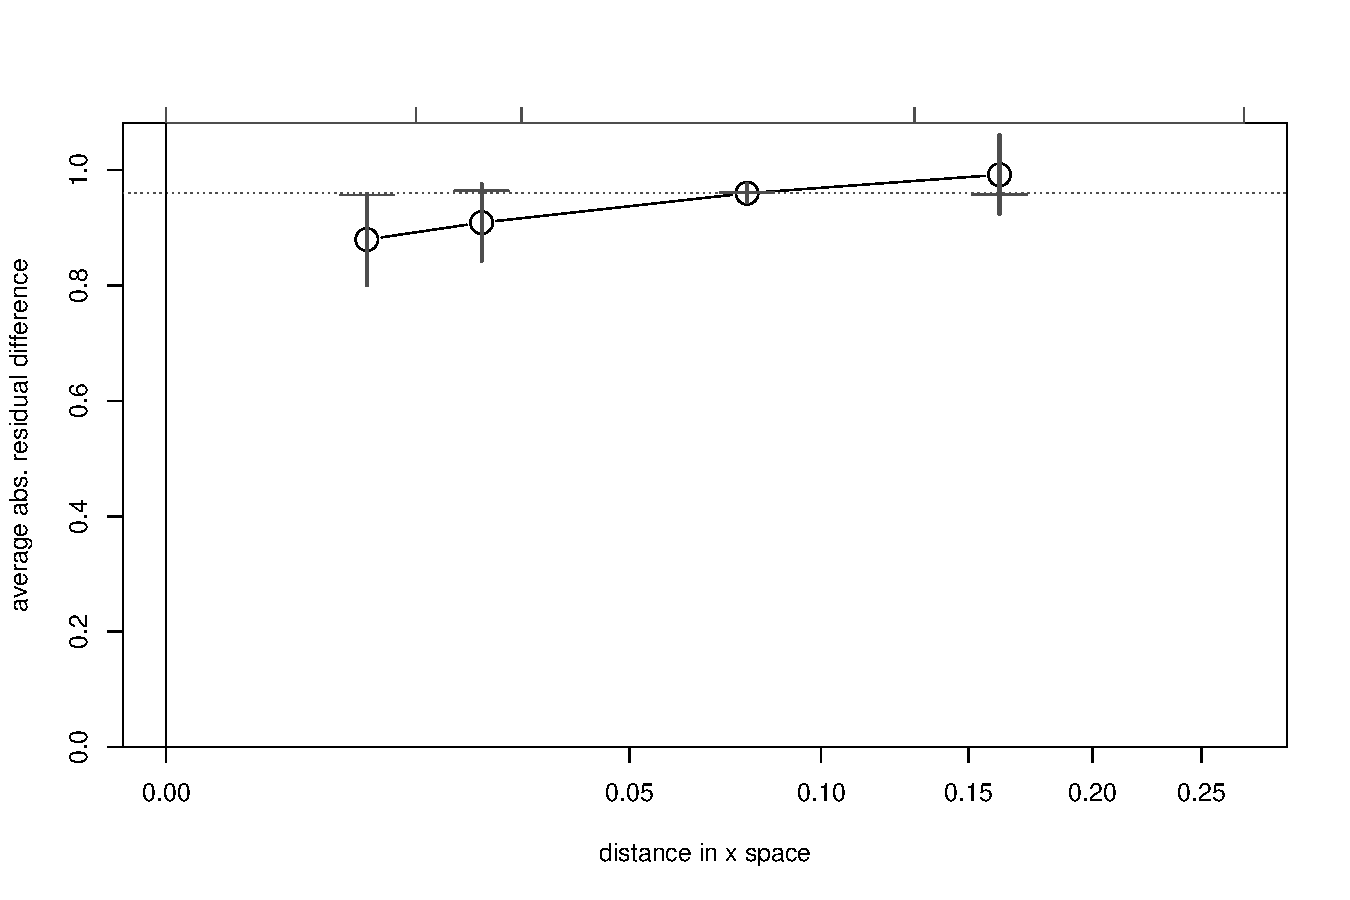
\includegraphics{regr-description-xdist}
\Efig{Residual differences against x distance}

This idea can also be used for a test of goodness of fit: The test
statistic 
$$
  T = \sum\nolimits_{k=1}^K \left((\wb d\sups R_k-\wb d)\big/\mbox{se}_k\right)^2
$$
should have a Chisquared distribution with $K-1$ degrees of freedom.
The test is calculated by the function \texttt{xdistResscale} along with
the mean distances and mean residual differences.

\subsection{Sequence Plot}
Residuals are plotted against the sequence number in the dataset in order
to show any trends and correlation that may be related to this sequence.



\subsection{Residuals against explanatory variables}
Plotting residuals against explanatory variables serves to detect
nonlinearities of the relation between the response and the variable in
question. 
For ordinary regression and some other models, they can show dependencies
of the scale of errors on the explanatory variables.

The plots are enhanced by smooths as discussed for the Tukey-Anscombe
plot. 
Also, a \textbf{reference line} is added that helps to decide whether a
transformation of the explanatory variable may help to remove any
non-linearity shown by the smooth.
Again, the reference line intends to connect points of equal response
values. Note, however, that they do not really align on a straight line
because of the contributions of the other terms in the model to the fit.
Therefore, the reference line connects points for which the sum of 
``component effect'' $\widehat\beta_j x^{(j)}$ plus residual is equal.
Note that the slope of the reference line is negative if the regressor has
a positive effect on the response.
The line is again useful for finding an adequate modification if a curved
smooth appears: If all parallels to the reference line cut the smooth only
once, a monotone transformation of the regressor can help. 
Otherwise, adding its square to the model may help.

Alternatively, the sums 
``component effect $\widehat\beta_j x^{(j)}$ plus residual''
may be used as the vertical axis instead of the
residuals for plotting. This display is usually called the 
``partial residual plot'' and can be obtained from \T{plot.regr}, too. 
It is related to the plots shown by default in the same way as the
response versus fitted plot is to the Tukey-Anscombe plot.

When \ul{transformed explanatory variables} appear in the model, the
residuals are plotted against the original values. The reason is as
follows: If any curvature is detected, an improvement of the model may be
possible by transforming the variable shown. It is then more natural
to search for an enhancement of the original transformation rather than 
a transformation of transformed values, and this should be easier if 
the original scale is used.
If this appears to be unsuitable in a given application, the user
may store the transformed variable under a new name and then use 
this new variable in the model formula, or specify the transformed 
variable in the call to \T{plot}.

Residuals may be plotted against any variables using an additional function 
\T{plresx}. The function \T{plres2x} displays residuals and two
(explanatory) variables in a special type of 3d plot. This serves to 
\ul{check for interactions.}

\subsection{Residuals for an ordinal or binary response}
Ordinal regression models are best specified by introducing the idea of a 
``latent response variable'' $Z$, which is continuous and follows a linear
relationship with the explanatory variables. 
The response $Y$ is considered to be a classification of $Z$ into $k$
classes of possibly unequal width. The most well-known model specifies a 
logistic distribution for the error term in the linear model for $Z$.
Then, the coefficients and the thresholds or class limits are estimated by
maximum likelihood. This is implemented in the function \T{polr} 
(proportional odds linear regression) of the \T{MASS} package, 
which is the function invoked by \T{regr} for ordinal regression.

Residuals for this model may be defined by considering the conditional
distribution of the latent variable $Z$, given the observation $Y$ and the
explanatory variables. This is a logistic distribution with parameters
given by the model, restricted to the class of $Z$ given by the observed
$Y$. Residuals are defined as the median of this distribution, and 
it may help to characterize the uncertainty about the latent residuals by 
the quartiles of the conditional distribution.
The plots show the interquartile range by a vertical line and the median,
by a horizontal tick on them. (The vertical line is not shown if the 
probability observed $Y$ is either too low or too high, see argument
\T{condprobrange}.)
In addition, random numbers according to the conditional distribution are
shown. 

Note that this definition may not have appeared in the literature yet.

\Bfig
\begin{Schunk}
\begin{Soutput}
[1] "plot.regr done"
\end{Soutput}
\end{Schunk}
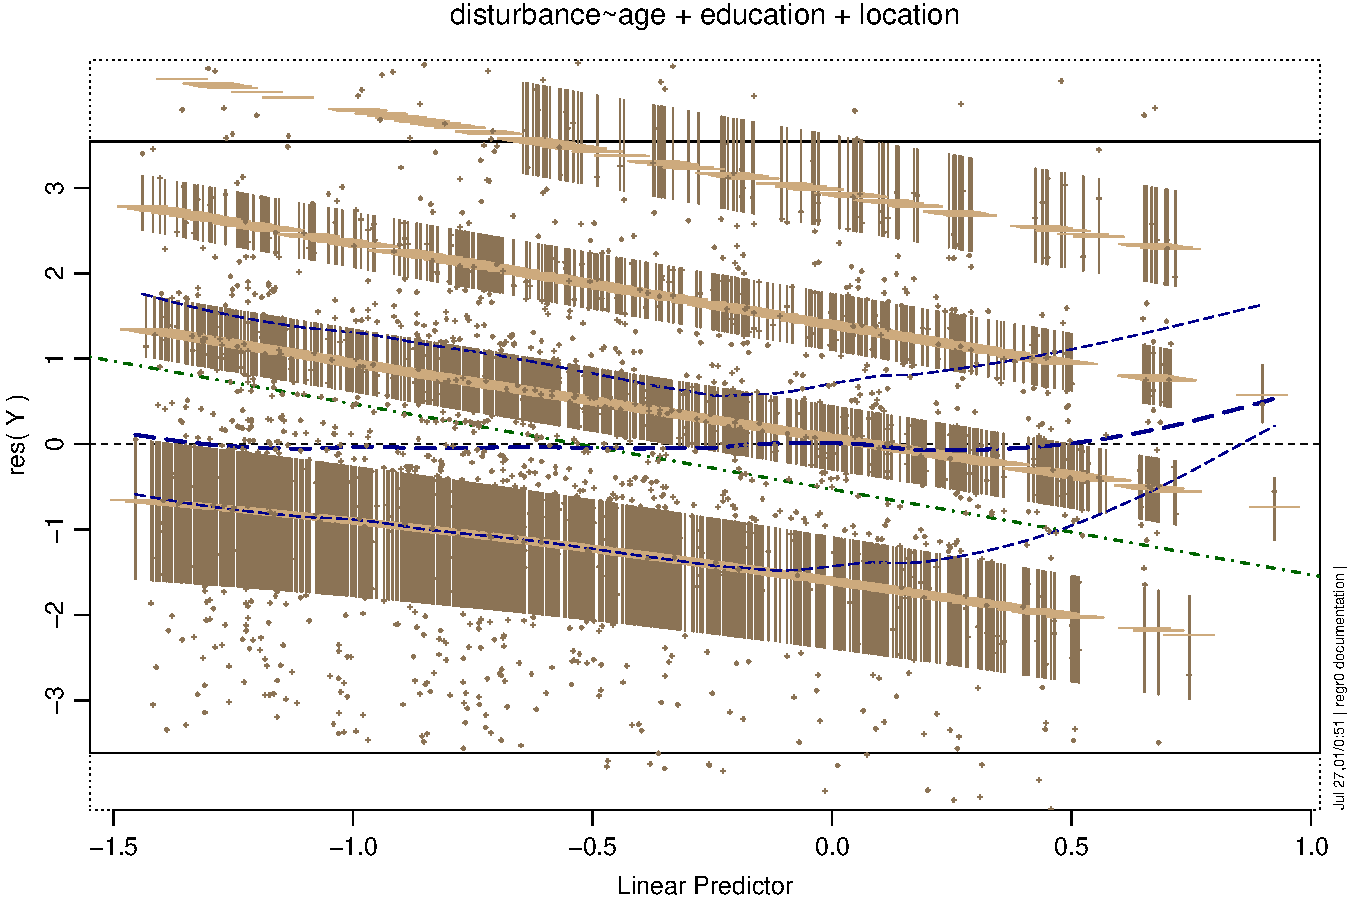
\includegraphics{regr-description-taordered}
\Efig{\label{fig:taordered}
  Tukey-Anscombe plot for ordered regression
  }
  
  
\subsection{Residuals for censored responses}
If response values are censored, so are the residuals. In the same spirit
as for the case of ordered responses, it is straightforward to calculate 
a conditional distribution, given the fitted value and the censoring value,
for each residual. This can again be plotted by showing quartiles.

\subsection{Residuals for the Cox model}

The Cox proportional hazards model, the most frequently used model in
survival analysis, is a semi-parametric model. There is no obvious meaning
of the notion residual in this context. 
The Cox-Snell residuals $R_{CS}$ are defined in a way that they alsways
follow an exponential distribution. 
Since this is an unususal law for residuals, it is convenient to transform
them such that they then obey a standard normal distribution,
\[
  R = \Phi\inv\fn{1-\exp\fn{-R_{CS}}}
\;.\]
Note that it is useless to draw a QQ-plot of these residuals, since they
obey the normal law by construction. (? !!!)
They should are are plotted against the linear predictor values 
(Tukey-Anscombe plot) and against the explanatory variables.


\subsection{Residual plots for multivariate regression.}
For multivariate regression, the plots corresponding to each target
variable should be examined. 
They are arranged such that the same type of plot for the different
response variables are grouped together, and a matrix of plots is produced
for residuals against explanatory variables.
In addition, the qq-plot of Mahalanobis norms of residuals is shown as well
as the scatterplot matrix of residuals.

\Vneed{30mm}
\section{Further Plotting Functions}
\subsection{Scatterplot Matrices}
Scatterplot matrices are produced by the \T{pairs} function.
In \T{regr0}, there is a function with more flexibility, called
\T{plmatrix}.
\begin{itemize}
\item 
  The set of variables shown horizontally and vertically need not be the
  same. \T{plmatrix} can be used to show the dependence of several 
  response variables (vertical axes) on several explanatory ones
  (horizontal axes).
\item
  A traditional square scatterplot matrix can be split to avoid
  tiny panels -- this is even done by default. For example, if 
  a scatterplot matrix of 15 variables is needed, 
  \T{plmatrix} produces by default 6 pages of graphical output,
  the first one showing the % of the first 6 variables 
  upper corner of the lower triangle of the scatterplot matrix,
  the second, variables 7 to 11 against 1 to 6, the third, 
  7 to 11 against 7 to 12, and so on, until the whole lower triangle
  of the full scatterplot matrix is presented.
\item
  The first argument can be a formula. If it contains a left hand side,
  then the respective variables will be shown last in a scatterplot
  matrix. This is convenient since then, the target variable will appear as
  the vertical axis in the last row of plots, such that its (``marginal'')
  dependence on the explanatory variables can be seen in the usual way.
\item
  Plotting characters and colors may be specified directly (instead of 
  writing a panel function).
\item
  If only one x and one y variable is given, then a regular plot appears.
  Therefore, \T{plmatrix} can be used to generate a plot with specified
  plotting symbols (possibly labels of more than one character each),
  colors and symbol sizes.
\end{itemize}

\Bfig
\begin{Schunk}
\begin{Soutput}
[1] "plmatrix: done"
\end{Soutput}
\end{Schunk}
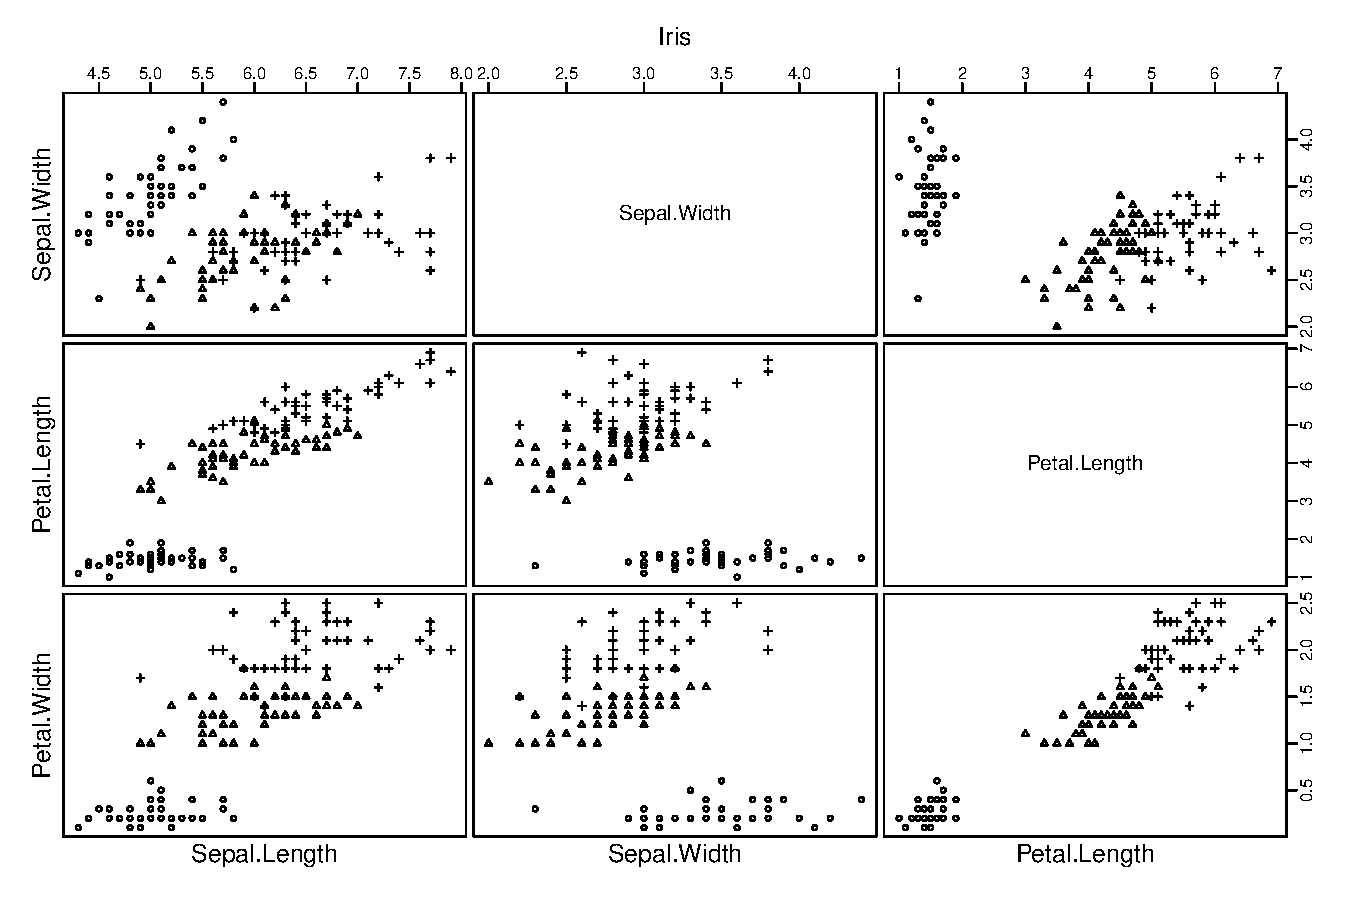
\includegraphics{regr-description-plmatrix}
\Efig{\label{fig:plmatrix}
  Plot matrix for iris data
}

\subsection{Multiboxes}

When a quantitative variable is plotted against a grouping variable
(factor), the usual \T{formula} method of the \T{plot} function produces
multiple box plots, one for each group. When there are many observations
per group, a box plot constitutes a very rough image of the distributeion.
The ``multibox plot'' is a refinement that shows the distribution in more
detail. 

The idea is to combine the virtues of the box plot, which is based on the
quartiles, with those of a histogram that depicts the density of the
distribution. 
Essentially, a histogram is drawn using quantiles as class limits.
The number of quantiles -- or the number of classes -- used should be
adapted to the number of observations to be represented.
For moderate sample sizes, ``octiles'' appear suitable.

\Bfig
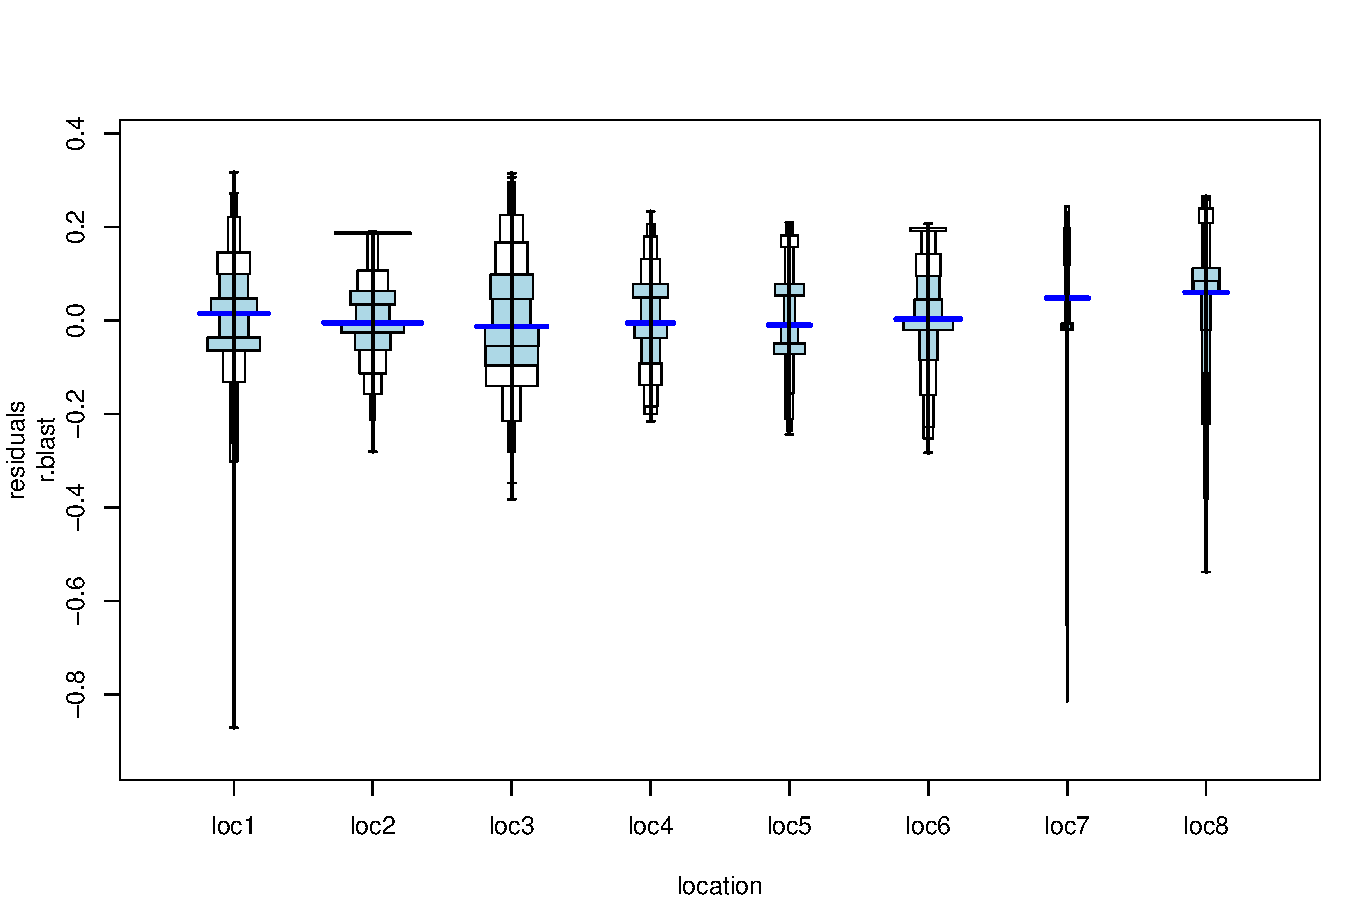
\includegraphics{regr-description-mboxes}
\Efig{\label{fig:mbox}
  Multibox plot of residuals for the explanatory factor \T{location}
  }
Since raw quantiles may be poor characterizations for discrete data,
``interpolated quantiles'' are used as class limits.

The multiboxes in Figure \ref{fig:mboxes} resemble a well-known kind of
presentation of age distributions. Often, these displays are asymmetric,
showing the age distribution of the two genders on the two sides.
In much the same way, asymmetric multibox plots can be drawn to visualize
the relationship of the continuous variable with any binary variable.
Figure \ref{fig:mboxes2} shows the distribution of ....

\Bfig
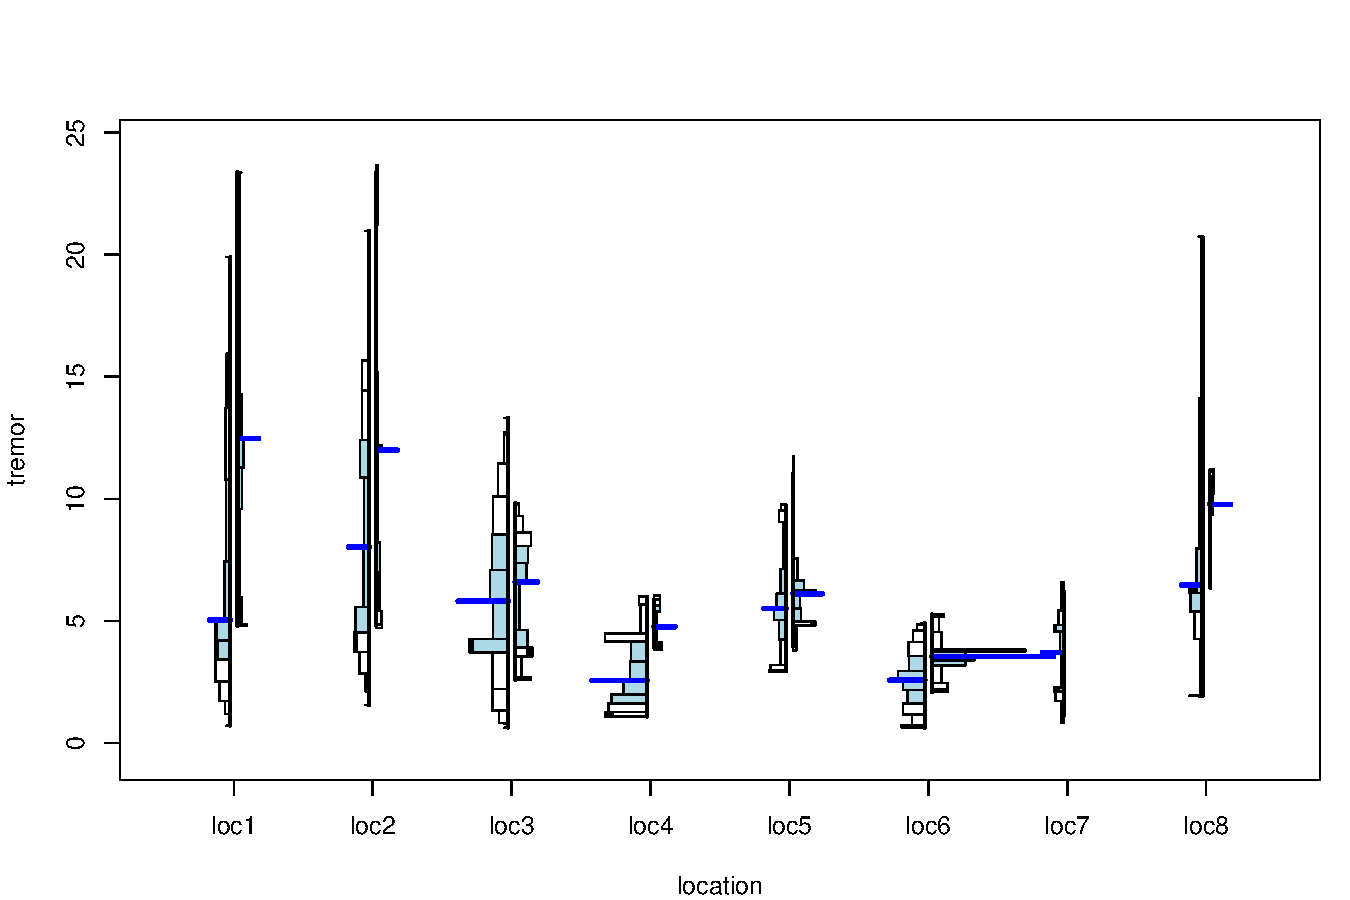
\includegraphics{regr-description-mboxes2}
\Efig{\label{fig:mboxes2}
  Target variable \T{tremor} related to factor{location} and binary variable
  \T{charge>5}
}

%% =================================================================
\Vneed{50mm}
\section{Miscellaneous and Utility Functions}
\subsection{Transformation: Started Logarithm}
The logarithmic transformation is very useful for quantitative variables. 
In fact, it should appear more often than not, since it is the
``first aid transformation'' for amounts and concentrations and should
therefore be applied to most quantitative variables by default.

Now, amounts and concentrations may be zero (exactly or recorded as such),
and the logarithm of 0 is \texttt{-Inf}. 
A pragamtic way out of this problem often consists of adding a constant
to the variable before taking logs. 
Generally, this and other ideas to avoid the \texttt{-Inf} as a transformed
value are called ``started logs'' according to John Tukey.

\texttt{regr0} includes a function \texttt{logst} that is based on the
following ideas:
\begin{itemize}
\item 
The modification should only affect the values for ``small'' arguments.
\item
What is ``small'' should be determined in connection with the non-zero 
values of the original variable, since it should behave well (be
equivariant) with respect to a change in the ``unit of measurement''.
\item
The function must remain monotone, and it should remain (weakly) convex.
\end{itemize}

The function \texttt{logst} implements these criteria in the following way: 
The shape is determined by a threshold $c$ at which -- coming from above --
the log function switches to a linear function with the same slope at this
point. This is obtained by
$$
  g(x) = \left\{\begin{array}{ll}\log_{10}(x) & \mbox{if\ \ } x\ge c\\
         \log_{10}(c) - (c-x)/(c\log(10)) & \mbox{if\ \ } x< c
         \end{array}\right.
$$
The threshold $c$ is set to
$ c = q_1^{1+r}/q_3^r$, where $q_1$ and $q_3$ are the quartiles of the 
positive data and $r$ is a tuning constant. 
The default of $r$ is 1 and leads to an expected
percentage of about 2\% of the data below $c$ for log-normal data.

It is certainly useful to inspect a graph of the function, as drawn in 
\texttt{example(logst)}.


\subsection{Documentation}
For a data analysis, it is often useful to save graphical displays in 
documents or on paper. In an extended data analysis, one can easily lose
control over the precise content of the different plots.
\T{regr0} provides some help for keeping track.
\begin{itemize}
\item 
  Every graphical display generated by a graphical function from the
  package gets a ``stamp'' in the lower right corner that indicates date
  and time of its creation and, if specified by the user before that 
  time point, a project title and a step name (by writing\\
  \T{userOptions(project=projecttitle, step=stepname)}).\\
  (This stamp can of course be suppressed for producing publication
  graphics.) 
\item
  Data sets may be documented by attaching two attributes, \T{tit} and 
  \T{doc} -- title and description --, which will be printed with
  numerical output if desired.
\end{itemize}

\subsection{Subsetting Data}
If observations (rows) of a data.frame are to be deleted, the usual
R-function \T{subset} is useful. The package slightly modifies it to make
sure that the attributes -- most importantly the documentation by
\T{tit} and \T{doc} (see the preceding subsection) are passed along.

There is an additional function \T{dropdata} which allows for dropping
observations or variables based on their names.

\subsection{Multiple Frames}
Function \T{mframe} splits the screen by calling \T{par(mfrow=...)}.
It adds flexibility and sets other defaults for margin widths and the like. 
\\[10mm]

{\small
\Tit{This is the end} of the story for the time being. I hope that you will
get into using \T{regr0} and have good success with your data analyses.
Feedback is highly appreciated.

Werner Stahel, \T{stahel at stat.math.ethz.ch}
}
\end{document}

%%% Local Variables: 
%%% mode: latex
%%% TeX-master: t
%%% End: 
